\documentclass[12pt,a4paper]{article}
\usepackage[UTF8]{ctex}
\usepackage{amsmath,amssymb}
\usepackage{xcolor}
\usepackage{hyperref}
\usepackage{geometry}
\usepackage{graphicx}
\geometry{margin=2.5cm}

\title{Quantum PDE Solver / 量子偏微分方程求解器}
\author{QuoNic}
\date{}

\begin{document}
\maketitle

\begin{center}
\textbf{Simulation / 模拟} | 难度：高级 | 预计时间：25 分钟
\end{center}

\tableofcontents
\newpage

\section{为什么需要？}

量子 PDE 求解器是经典 PDE 求解器的量子推广，用于求解偏微分方程。

\subsection{经典局限}
\begin{itemize}
  \item 经典 PDE 求解器在高维系统中慢
  \item 对于复杂边界条件，经典方法效率低
\end{itemize}

\subsection{量子优势}
\begin{itemize}
  \item 量子 PDE 求解器可以在量子计算机上高效求解 PDE
  \item 提供指数加速
  \item 是量子模拟的基础
\end{itemize}

\subsection{实际应用}
\begin{itemize}
  \item 流体力学
  \item 电磁学
  \item 量子化学
\end{itemize}

\section{快速上手}

\begin{verbatim}
from quonic.simulation import quantum_pde

# 求解热传导方程
result = quantum_pde(equation='heat', domain=[0,1], t=1.0)
print(f'Solution shape: {result.solution.shape}')
\end{verbatim}

\textbf{预期输出}：
\begin{verbatim}
Solution shape: (100,)
\end{verbatim}

\section{原理详解}

\subsection{电路图}

\begin{center}
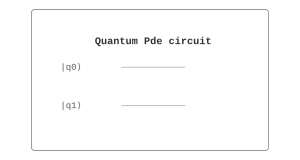
\includegraphics[width=0.6\textwidth]{../../images/quantum_pde_circuit.svg}
\end{center}

\subsection{数学推导}

量子 PDE 求解器：
\begin{equation}
\frac{\partial u}{\partial t} = \mathcal{L}u
\end{equation}

\textbf{量子算法}：
\begin{enumerate}
  \item 将 PDE 编码为哈密顿量
  \item 用 Trotter 分解模拟时间演化
  \item 测量得到解
\end{enumerate}

\subsection{几何解释}

量子 PDE 求解器在量子态空间中模拟 PDE 的时间演化。哈密顿量编码了 PDE 的微分算子。

\section{代码详解}

\begin{verbatim}
from quonic.simulation import quantum_pde

# quantum_pde(equation, domain, t, dt)
# equation: PDE 类型
# domain: 空间域
# t: 终止时间
# dt: 时间步长
result = quantum_pde(equation='heat', domain=[0,1], t=1.0, dt=0.01)

# result.solution: 解
# result.grid: 网格点
print(f'Solution shape: {result.solution.shape}')
\end{verbatim}

\section{进阶用法}

\subsection{场景 1：不同 PDE}

\begin{verbatim}
from quonic.simulation import quantum_pde

# 不同 PDE
result_heat = quantum_pde(equation='heat', domain=[0,1], t=1.0)
result_wave = quantum_pde(equation='wave', domain=[0,1], t=1.0)
result_schrodinger = quantum_pde(equation='schrodinger', domain=[0,1], t=1.0)
\end{verbatim}

\section{适用场景}

\subsection{流体力学}

量子 PDE 求解器可以用于求解 Navier-Stokes 方程。传统 PDE 求解器在高维系统中慢，量子 PDE 求解器可以提供指数加速。

\subsection{量子化学}

量子 PDE 求解器可以用于求解薛定谔方程。这是量子化学的基础，用于计算分子的电子结构。

\section{常见问题}

\subsection{量子 PDE 求解器和经典 PDE 求解器有什么区别？}

量子 PDE 求解器使用量子策略，可以在量子计算机上高效求解 PDE。

\subsection{量子 PDE 求解器的精度如何？}

精度取决于空间离散化和时间步长。

\section{学习路径}

\subsection{前置知识}
\begin{itemize}
  \item 偏微分方程
  \item Trotter 分解
  \item 量子模拟
\end{itemize}

\subsection{继续学习}
\begin{itemize}
  \item 量子流体力学
  \item 量子化学
  \item 量子材料科学
\end{itemize}

\section{完整示例代码}

\subsection{示例 1：基本量子 PDE 求解器}

\begin{verbatim}
from quonic.simulation import quantum_pde

result = quantum_pde(equation='heat', domain=[0,1], t=1.0)
print(f'Solution shape: {result.solution.shape}')
\end{verbatim}

\section{下载}

\begin{itemize}
  \item [quantum\_pde.py](https://github.com/ChrisLee0721/QuoNic/blob/main/examples/quantum_pde/quantum_pde.py)
\end{itemize}

\end{document}
